\documentclass{ximera}

\graphicspath{{./content/03_03_higher_order_partials/graphics/}{./graphics/}}

\title{Higher Order Partial Derivatives}
\author{Melissa Lynn}
\outcome{Compute higher order partial derivatives, and understand their geometric significance. Understand how to apply Clairaut's theorem.}

\begin{document}
\begin{abstract}
\end{abstract}
\maketitle


Back in single variable Calculus, we were able to use the second derivative to get information about a function. For instance, the second derivative gave us valuable information about the shape of the graph. More specifically, we could use the second derivative to determine the concavity.
\begin{itemize}
\item If $f''(x)>0$ on an interval, then the graph of $f$ is concave up on that interval.
\item If $f''(x)<0$ on an interval, then the graph of $f$ is concave down on that interval.
\item If $f''$ changes signs at a point, then the graph of $f$ has an inflection point at that point.
\end{itemize}
Furthermore, we were able to use second derivative in conjunction with roots of the first derivative to find local maxima and minima. We could also think about the second derivative as the rate-of-change of a rate-of-change, or describing some sort of acceleration or deceleration.

Since the second derivative contains so much useful information, we would like to come up with a way to define second derivatives for multivariable functions! At first, this might seem simple: just take the derivative of the derivative. But when we took the total derivative of a multivariable function $f:\mathbb{R}^m\rightarrow\mathbb{R}^n$, we got a matrix of partial derivatives, and it's not at all clear how we would differentiate a matrix.

For now, we'll settle for defining second order partial derivatives, and we'll have to wait until later in the course to define more general second order derivatives. Fortunately, second order partial derivatives work exactly like you'd expect: you simply take the partial derivative of a partial derivative.

\section*{Higher Order Partials}

\begin{example}
Consider the function $f(x,y) = 2x^2+4xy-7y^2$. We'll start by computing the first order partial derivatives of $f$, with respect to $x$ and $y$.
\begin{align*}
f_x(x,y) &= \answer{6x+4y}\\
f_y(x,y) &= \answer{4x-14y}
\end{align*}
We can then compute the second order partial derivatives $f_{xx}$ and $f_{yy}$ by differentiating with respect to $x$ again, and with respect to $y$ again.
\begin{align*}
f_{xx}(x,y) &= \answer{6}\\
f_{yy}(x,y) &= \answer{-14}
\end{align*}
However, this isn't the only way that we could take second order partial derivatives! We could differentiate with respect to $x$ first, and with respect to $y$ second, to get $f_{xy}$. We could also differentiate with respect to $y$ first, and with respect to $x$ second, to get $f_{yx}$.
\begin{align*}
f_{xy}(x,y) &= \answer{4}\\
f_{yx}(x,y) &= \answer{4}
\end{align*}
Notice that we got the same result for $f_{xy}$ and $f_{yx}$, so it didn't end up mattering what order we took these derivatives in. In turns out that this is not a coincidence, and it's a consequence of Clairaut's Theorem, which we'll talk about in the next section.
\end{example}

There are a few different ways that we can denote second order partials. We can denote the second order partial of $f$ that we get by differentiating with respect to $x$ twice as any of the following.
\[
f_{xx}(x,y)\hspace{1cm}\frac{\partial}{\partial x}\left(\frac{\partial f}{\partial x}\right)\hspace{1cm} \frac{\partial^2 f}{\partial x^2}
\]
For the second order partial of $f$ that we get by differentiating with respect to $x$ first, then differentiating with respect to $y$, we denote this as below.
\[
f_{xy}(x,y)\hspace{1cm}\frac{\partial}{\partial y}\left(\frac{\partial f}{\partial x}\right)\hspace{1cm} \frac{\partial^2 f}{\partial y\partial x}
\]
To remember what order to take these derivatives for all of these notations, start with the variable closest to $f$, and work your way out.

We can similarly define and compute third order partials, fourth order partials, and so on.

\begin{example}
Consider the function $f(x,y,z) = xy^2z^3 + x^2z$. Compute each of the following.
\begin{align*}
f_{xx}(x,y,z) &= \answer{2z}\\
f_{xz}(x,y,z) &= \answer{3y^2z^2+2x}\\
\frac{\partial^2 f}{\partial x\partial z}(x,y,z) &= \answer{3y^2z^2+2x}\\
\frac{\partial^3 f}{\partial x^2\partial y}(x,y,z) &= \answer{0}\\
\frac{\partial^3 f}{\partial x\partial y\partial x}(x,y,z) &= \answer{0}
\end{align*}
\end{example}

\section*{Clairaut's Theorem}

In previous examples, we've seen that it doesn't matter what order you use to take higher order partial derivatives, you seem to wind up with the same answer no matter what. This isn't an amazing coincidence where we randomly chose functions that happened to have this property; this turns out to be true for many functions. Clairaut's Theorem gives us this result.

\begin{theorem}
(Clairaut's Theorem) Suppose we have a function $f:D\subset \mathbb{R}^n\rightarrow \mathbb{R}$. Suppose further that \emph{all} of the second order mixed partial derivatives of $f(x_1,...,x_n)$ exist and are continuous on an open disc around $\vec{a}\in D$. Then, for any $x_i$ and $x_j$,
\[
f_{x_ix_j}(\vec{a})=f_{x_jx_i}(\vec{a}).
\]
\end{theorem}

We have a similar result for even higher order partial derivatives. Before we state that result, we'll introduce a new definition to make it easier to describe how ``nice'' functions are.

\begin{definition}
A function $f:\mathbb{R}^n\rightarrow\mathbb{R}^m$ is of class $\mathcal{C}^k$ if all of the partial derivatives of $f$ up to and including the $k$th order exist and are continuous.

If $f$ is of class $\mathcal{C}^k$ for all $k$, then we say $f$ is of class $\mathcal{C}^\infty$.

If $f$ is continuous, we say $f$ is of class $\mathcal{C}^0$.
\end{definition}

We'll often write this as $f\in\mathcal{C}^3$ and say ``$f$ is $\mathcal{C}$ three,'' for example, if $f$ is of class $\mathcal{C}^3$.

\begin{problem}
If $f(x,y) = x^2+y^2+2xy$, which of the following are true? Select all that apply.
\begin{selectAll}
\choice[correct]{$f$ is $\mathcal{C}^0$.}
\choice[correct]{$f$ is $\mathcal{C}^1$.}
\choice[correct]{$f$ is $\mathcal{C}^2$.}
\choice[correct]{$f$ is $\mathcal{C}^3$.}
\choice[correct]{$f$ is $\mathcal{C}^\infty$.}
\end{selectAll}
\end{problem}

We can generalize Clairaut's Theorem to $k$th order derivatives for $\mathcal{C}^k$ functions.

\begin{theorem}
If $f$ is $\mathcal{C}^k$, then the $k$th order mixed partials can be computed in any order.
\end{theorem}

For example, if $f$ is $\mathcal{C}^{12}$, we have
\begin{align*}
f_{xyxyzyzzxyxz}&=f_{xxxxyyyyzzzz}\\
&=f_{xyzxyzxyzxyz}.
\end{align*}

\begin{problem}
If $f$ is $\mathcal{C}^5$, which of the following are guaranteed to be equal to $f_{zzyzx}$? Select all that apply,
\begin{selectAll}
\choice{$f_{xxzxy}$}
\choice[correct]{$f_{xyzzz}$}
\choice[correct]{$f_{xzzzy}$}
\choice[correct]{$f_{zzxzy}$}
\choice{$f_{yyzyx}$}
\end{selectAll}
\end{problem}

\section*{Geometric Significance}

Remembering back to single variable calculus, we could use the first and second derivatives of a function to figure out the shape of the graph.

More precisely, we used the first derivative to determine where a function was increasing and where it was decreasing. If $f'(x)>0$ on some interval, then $f(x)$ is increasing on that interval. If $f'(x)<0$ on some interval, then $f(x)$ is decreasing on that interval.

\begin{image}
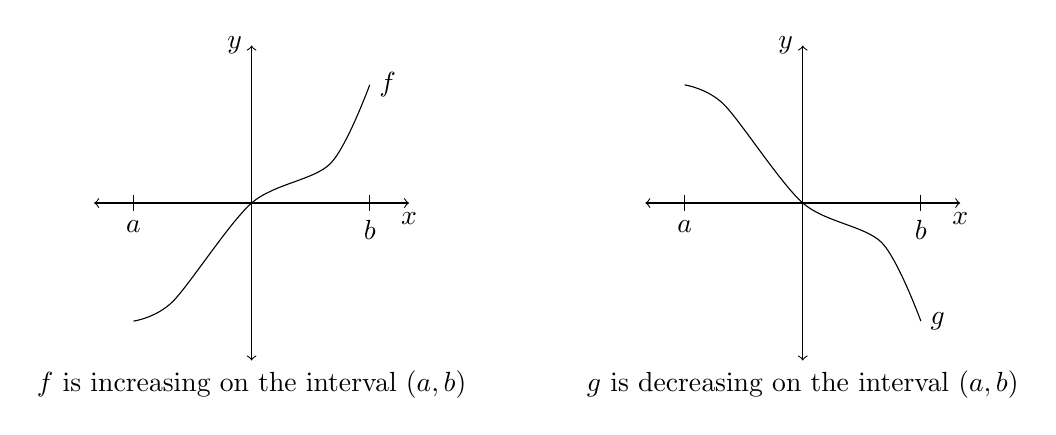
\begin{tikzpicture}
\draw[<->] (-2,0) -- (2,0)node[below] {$x$};
\draw[<->] (0,-2) -- (0,2)node[left] {$y$};
\draw plot [smooth, tension = .5] coordinates {(-1.5,-1.5) (-1, -1.25) (0,0) (1,.5) (1.5,1.5)};
\node[anchor = west]  at (1.5,1.5)  {$f$};
\draw (-1.5,.1) -- (-1.5,-.1)node[below]{$a$};
\draw (1.5,.1) -- (1.5,-.1)node[below]{$b$};
\node[anchor = north]  at (0,-2)  {$f$ is increasing on the interval $(a,b)$};

\begin{scope}[xshift = 7cm]
\draw[<->] (-2,0) -- (2,0)node[below] {$x$};
\draw[<->] (0,-2) -- (0,2)node[left] {$y$};
\draw plot [smooth, tension = .5] coordinates {(-1.5,1.5) (-1, 1.25) (0,0) (1,-.5) (1.5,-1.5)};
\node[anchor = west]  at (1.5,-1.5)  {$g$};
\draw (-1.5,.1) -- (-1.5,-.1)node[below]{$a$};
\draw (1.5,.1) -- (1.5,-.1)node[below]{$b$};
\node[anchor = north]  at (0,-2)  {$g$ is decreasing on the interval $(a,b)$};
\end{scope}
\end{tikzpicture}
\end{image}

We used the second derivative to determine the concavity of a function. If $f''(x)>0$ on an interval, then $f(x)$ is concave up on that interval. If $f''(x)<0$ on an interval, then $f(x)$ is concave down on that interval.

\begin{image}
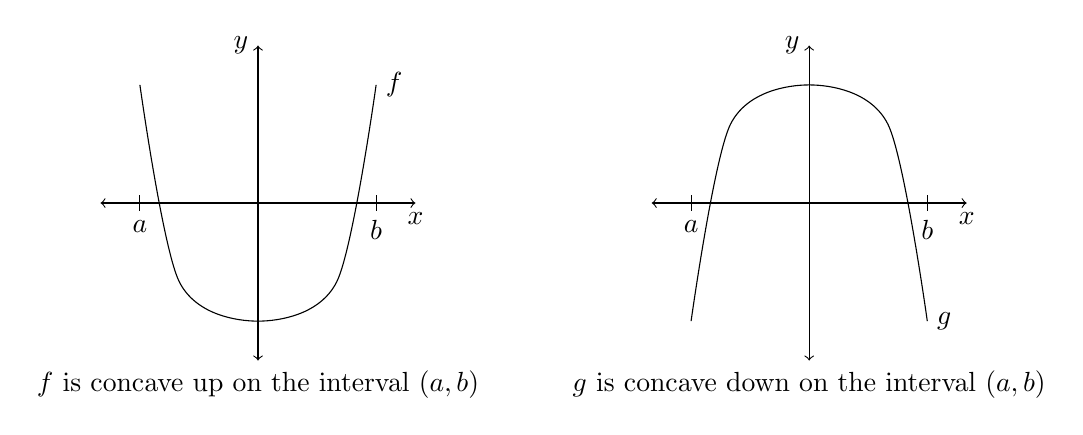
\begin{tikzpicture}
\draw[<->] (-2,0) -- (2,0)node[below] {$x$};
\draw[<->] (0,-2) -- (0,2)node[left] {$y$};
\draw plot [smooth, tension = .5] coordinates {(-1.5,1.5) (-1, -1) (0,-1.5) (1,-1) (1.5,1.5)};
\node[anchor = west]  at (1.5,1.5)  {$f$};
\draw (-1.5,.1) -- (-1.5,-.1)node[below]{$a$};
\draw (1.5,.1) -- (1.5,-.1)node[below]{$b$};
\node[anchor = north]  at (0,-2)  {$f$ is concave up on the interval $(a,b)$};

\begin{scope}[xshift = 7cm]
\draw[<->] (-2,0) -- (2,0)node[below] {$x$};
\draw[<->] (0,-2) -- (0,2)node[left] {$y$};
\draw plot [smooth, tension = .5] coordinates {(-1.5,-1.5) (-1, 1) (0,1.5) (1,1) (1.5,-1.5)};
\node[anchor = west]  at (1.5,-1.5)  {$g$};
\draw (-1.5,.1) -- (-1.5,-.1)node[below]{$a$};
\draw (1.5,.1) -- (1.5,-.1)node[below]{$b$};
\node[anchor = north]  at (0,-2)  {$g$ is concave down on the interval $(a,b)$};
\end{scope}
\end{tikzpicture}
\end{image}

Partial derivatives can give us similar information about the graph of a multivariable function, although the situation is a bit more nuanced. Let's consider a function $f:\mathbb{R}^2\rightarrow\mathbb{R}$, so we can visualize its graph. We've already seen that the partial derivative with respect to $x$ tells us how $f$ changes as $x$ changes.

More specifically, suppose $f_x(x,y_0)>0$ for $x$ in some open interval containing $x_0$. Then $f(x,y)$ is increasing as we move \emph{in the positive $x$-direction} from the point $(x_0,y_0)$. 

In the graph below, we can see that $f_x$ is positive near the point $(1,1)$, since the function increases as we move in the positive $x$ direction.

\youtube{DOBav9u7QDs}

Similarly, suppose $f_x(x,y_0)<0$ for $x$ in some open interval constaining $x_0$. Then $f(x,y)$ is increasing as we move in the positive $x$-direction from the point $(x_0,y_0)$.

In the graph below, we can see that $f_x$ is negative near the point $(-1,1)$, since the function increases as we move in the positive $x$ direction.

\youtube{pL2fhvhsoOU}

Suppose $f_x(x,y_0)=0$ for $x$ in some open interval constaining $x_0$. Then $f(x,y)$ is constant as we move in the positive $x$-direction from the point $(x_0,y_0)$.

In the graph below, we can see that $f_x$ is zero near the point $(0,1)$, since the function is constant as we move in the positive $x$ direction.

\youtube{co6uZeIDrSg}

It's also possible for $f_x$ to be zero at only an isolated point. In this case, the graph instantaneously flattens out in the $x$-direction. In the graph below, $f_x$ is zero at the point $(0,1)$.

\youtube{xzQARwQb3d8}

The partial derivative with respect to $y$, $f_y$, can tell us where $f$ is increasing, decreasing, or constant as we move in the positive $y$ direction.

Now, let's look at what the second-order partial derivatives tell us about the graph of the function $f(x,y)$. It shouldn't be too surprising that the sign of $f_{xx}$ tells us about the concavity of $f$ as we move in the positive $x$ direction.

In the graph below, $f_{xx}$ is positive at all points $(x,y)$.

\begin{image}
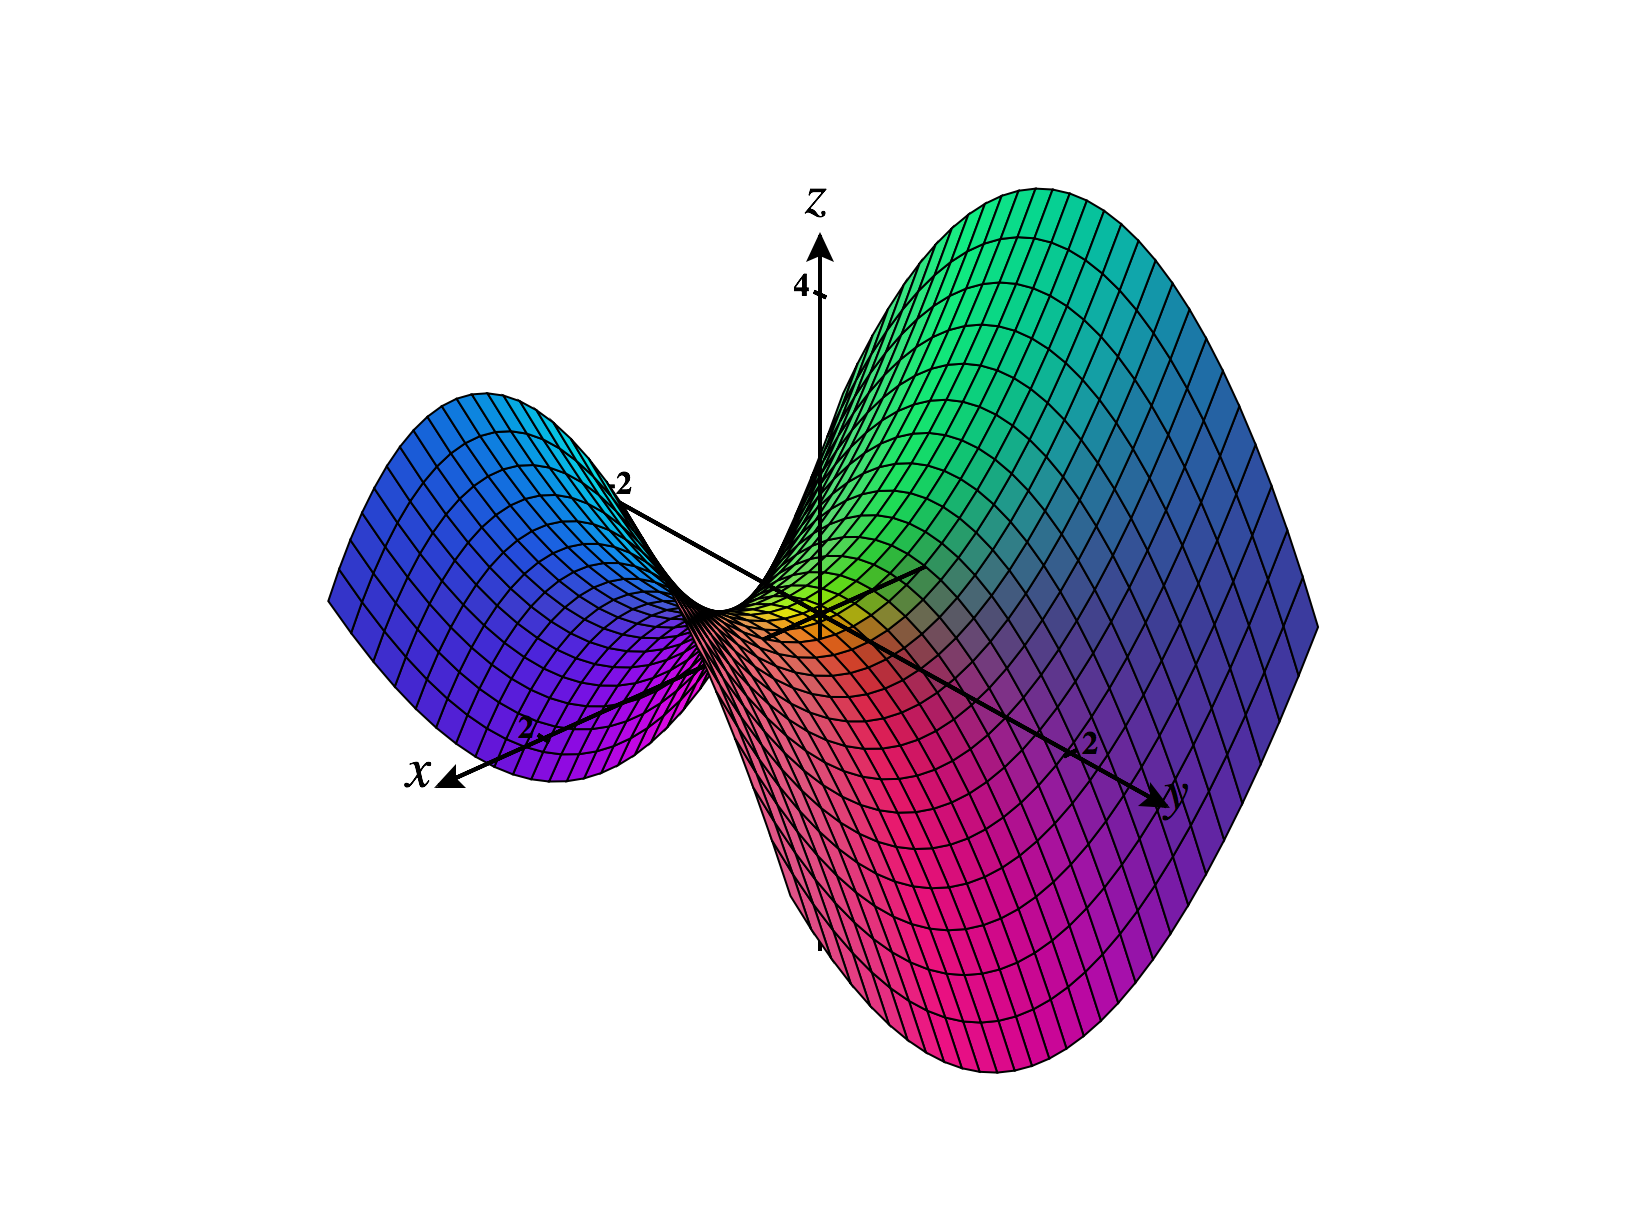
\includegraphics[width = \textwidth]{CalcPlot3D-fxx_pos}
\end{image}

Similarly, the sign of $f_{yy}$ tells us about the concavity of $f$ as we move in the positive $y$ direction. In the graph above, $f_{yy}$ is negative at all points $(x,y)$.

But what do the mixed partials, $f_{xy}$ and $f_{yx}$, tell us about the graph of $f$? Let's consider $f_{xy}$, which is the partial derivative of $f_x$ with respect to $y$. The partial derivative $f_x$ tells us the rate of change of $f$ as we move in the positive $x$ direction. Then, the partial derivative of $f_x$ with respect to $y$ tells us how $f_x$ changes as we move in the positive $y$ direction. That is, we look at how the rate of change in the $x$ direction changes as we move in the $y$ direction. This is a lot to unravel!

In the graph below, we can see that the slope in the $x$ direction is increasing as we move in the positive $y$ direction, so $f_{xy}$ is positive.

\youtube{jHzW6byRq_4}

We can similarly think of $f_{yx}$ as the change in $f_y$ as we move in the positive $x$ direction.

\youtube{ooj9Qpy79fY}

By Clairaut's theorem, for ``nice'' functions we'll always have $f_{xy}=f_{yx}$. This mixed partial tells us about how the graph of $f$ is ``twisted.''



\end{document}